\documentclass[t,24pt]{beamer}

\usepackage[english]{isodate}
\usepackage{KUstyle}
\usepackage{multicol}
\usepackage{amsthm}
\usepackage{amsfonts}
\usepackage{amsmath}
\usepackage{amssymb}
\usepackage{tikz}

\toplinje{Parallel LL Parsing}

\begin{document}

{
\setbeamertemplate{background}{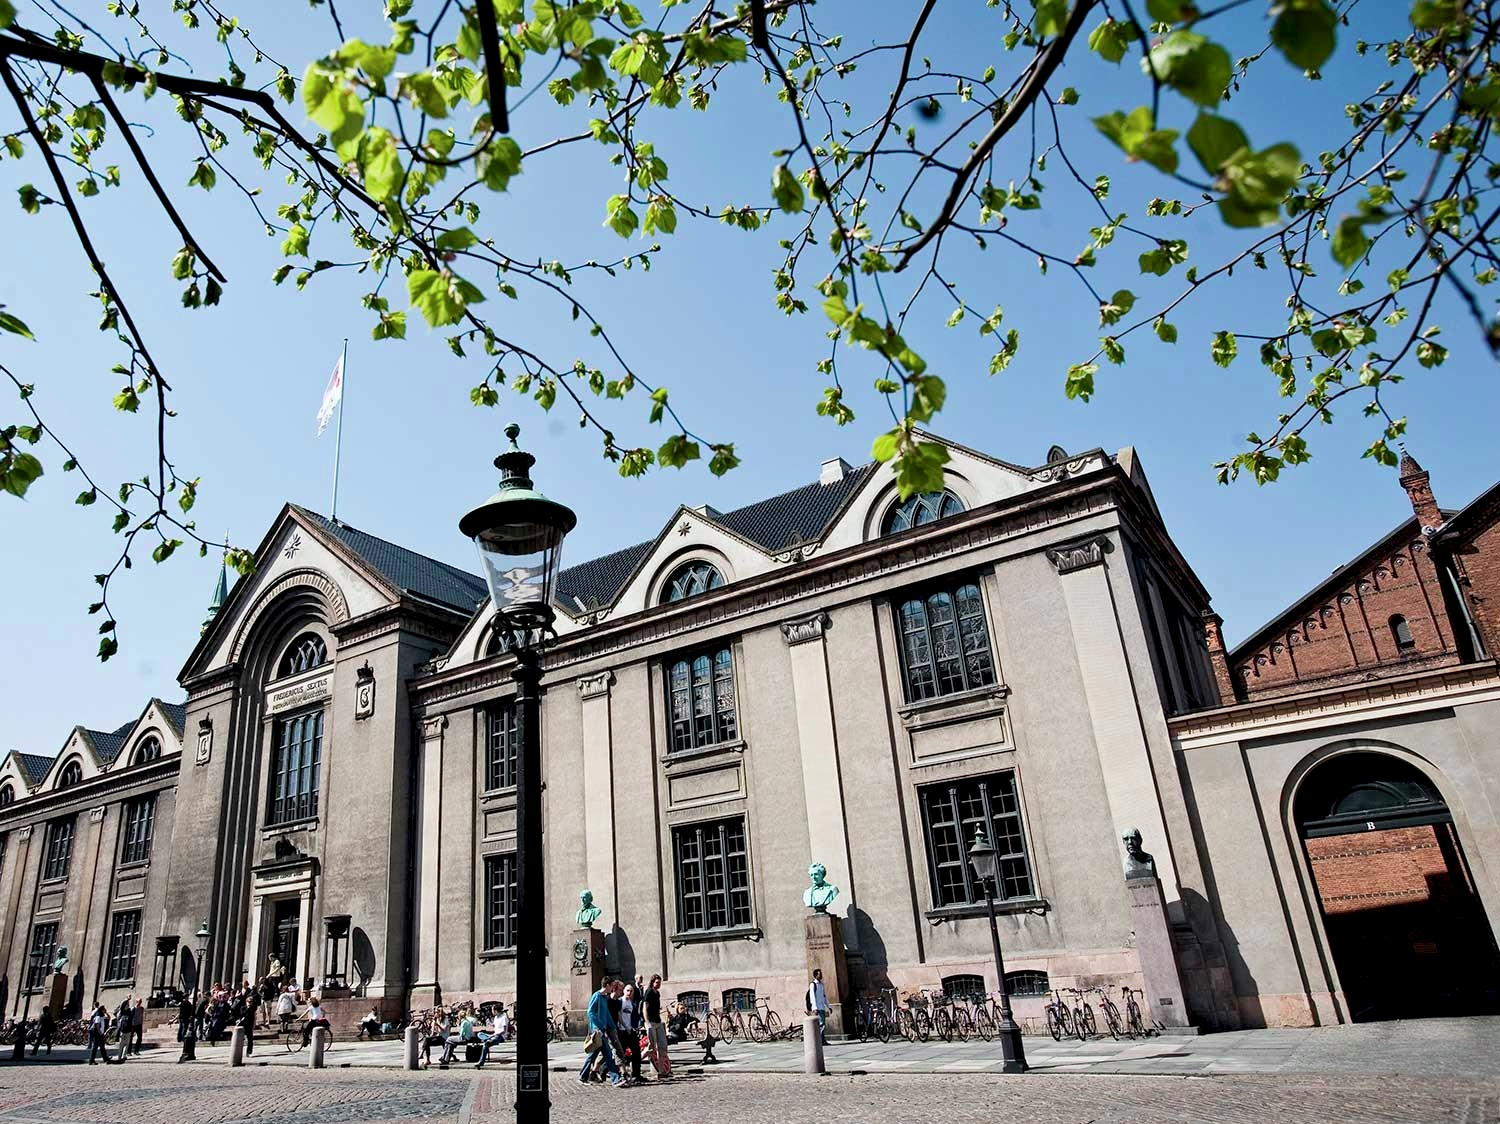
\includegraphics[width=\paperwidth,height=\paperheight]{images/frontpage.jpg}}
\begin{frame}
    \begin{textblock*}{\textwidth}(0.57\textwidth,0.1\textheight)
        \begin{beamercolorbox}[wd=6.4cm,ht=7.7cm,sep=0.5cm]{hvidbox}
            \fontsize{4}{10}\fontfamily{ptm}\selectfont \textls[200]{KØBENHAVNS UNIVERSITET}
            \noindent\textcolor{KUrod}{\rule{5.4cm}{0.4pt}}
        \end{beamercolorbox}
    \end{textblock*}
    \begin{textblock*}{\textwidth}(0.57\textwidth,0.1\textheight)
        \begin{beamercolorbox}[wd=6.4cm,sep=0.5cm]{hvidbox}
            \Huge \textcolor{KUrod}{Parallel Parsing}
            \vspace{0.5cm}
            \par
            \Large The Implementation of a Parallel LL Parser Generator
            \vspace{0.5cm}
            \par
            \normalsize William Henrich Due
            \vspace{0.1cm}
            \par
            30rd June 2023
        \end{beamercolorbox}
    \end{textblock*}
    \begin{textblock}{1}(14.2,11.44)
        
\includegraphics[width=1cm]{KU/KU-logo.png}
    \end{textblock}
\end{frame}
}

\begin{frame}[hvid,noframenumbering]
    \frametitle{LL parsing}
    Here is a LL(1) grammar.
    \begin{align*}
        1)\:\: T \to R \qquad 2)\:\: T \to aTc \qquad 3)\:\: R \to \varepsilon \qquad 4)\:\: R \to bR
    \end{align*}
    \begin{align*}
        \onslide<2->{(abc, T, ())} & \onslide<3->{\vdash (abc, aTc, 2)} \onslide<4->{\vdash (bc, Tc, 2)} \onslide<5->{\vdash (bc, Rc, (2, 1))} \\
                                   & \onslide<6->{\vdash (bc, bRc, (2, 1, 4))} \onslide<7->{\vdash (c, Rc, (2, 1, 4))}                         \\
                                   & \onslide<8->{\vdash (c, c, (2, 1, 4, 3))} \onslide<9->{\vdash (\varepsilon, \varepsilon, (2, 1, 4, 3))}
    \end{align*}
    \onslide<9->{Accepted! the string ``$abc$'' can be parsed.}
\end{frame}

\begin{frame}[hvid]
    \frametitle{LLP parsing}
    Augment the grammar.
    \begin{align*}
        0)\:\: T' \to \:\: \vdash T \dashv
    \end{align*}
    Now we parse the string ``$\vdash abc \dashv$'' instead.
    \begin{center}
        \begin{tabular}{ccccc}
            (\varepsilon ,\vdash) & $(\vdash, a)$ & $(a, b)$        & $(b, c)$             & $(c, \dashv)$               \\ \hline
            $(T',T\dashv,0)$      & $(T, Tc, 2)$  & $(T, R, (1,4))$ & $(Rc,\varepsilon,3)$ & $(\dashv, \varepsilon, ())$
        \end{tabular}
    \end{center}
\end{frame}
\begin{frame}[hvid]
    \frametitle{LLP parsing}
    \begin{center}
        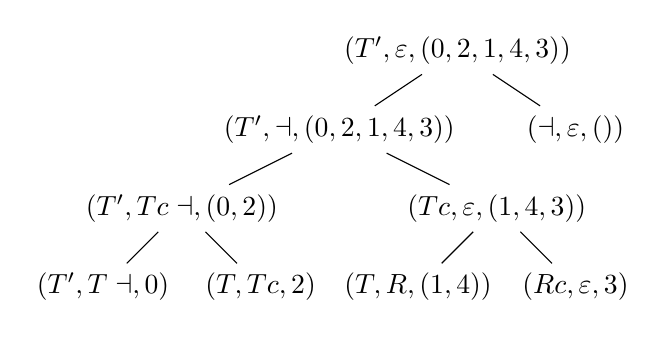
\begin{tikzpicture}[level distance=1cm,
                level 1/.style={sibling distance=3cm},
                level 2/.style={sibling distance=4cm},
                level 3/.style={sibling distance=2cm}]
            \node {$(T', \varepsilon, (0, 2, 1, 4, 3))$}
            child {node {$(T', \dashv, (0, 2, 1, 4, 3))$}
                    child {node {$(T',Tc\dashv, (0, 2))$}
                            child {node {$(T',T\dashv,0)$}}
                            child {node {$(T, Tc, 2)$}}
                        }
                    child {node {$(Tc, \varepsilon, (1,4,3 ))$}
                            child {node {$(T, R, (1,4))$}}
                            child {node {$(Rc,\varepsilon,3)$}}
                        }}
            child {node {$(\dashv, \varepsilon, ())$}};
        \end{tikzpicture}
    \end{center}
\end{frame}

% \begin{align*}
%     0)\:\: S' \to \: \vdash S \dashv \qquad 1)\:\: A \to \varepsilon \qquad 2)\:\: S \to aAa \qquad 3)\:\: A \to a
% \end{align*}
% \begin{table}[H]
%     \centering
%     \begin{tabular}{c|c|c|c}
%         & $\dashv$ & $a\dashv$ & $aa$ \\ \hline
%         $\vdash$ & & & $\{S\}$ \\\hline
%         $\vdash a$ & & $\{A\}$ & $\{A\}$ \\\hline
%         $aa$ & $\dashv$ & $\{a\}$ & 
%     \end{tabular}
% \end{table}
% Det efterfølgende er forskellige eksempler på slides
\begin{frame}[hvid]
    \frametitle{Liste med punkter}
    \begin{itemize}
        \item Punkt 1
        \item Punkt 2
              \begin{itemize}
                  \item Punkt 2.1
                  \item Punkt 2.2
              \end{itemize}
        \item Punkt 3
    \end{itemize}
\end{frame}

\begin{frame}[hvid]
    \frametitle{Slide med 2 kolonner}
    \begin{multicols}{2}
        \begin{itemize}
            \item Punkt 1
            \item Punkt 2
        \end{itemize}
        \vfill\null
        \columnbreak
        \begin{itemize}
            \item Punkt 3
            \item Punkt 4
            \item Punkt 5
        \end{itemize}
    \end{multicols}
\end{frame}

\begin{frame}[hvid]
    \frametitle{Slide med en kolonne og et billede}
    \begin{multicols}{2}
        \begin{itemize}
            \item Punkt 1
            \item Punkt 2
        \end{itemize}
        \vfill\null
        \columnbreak
        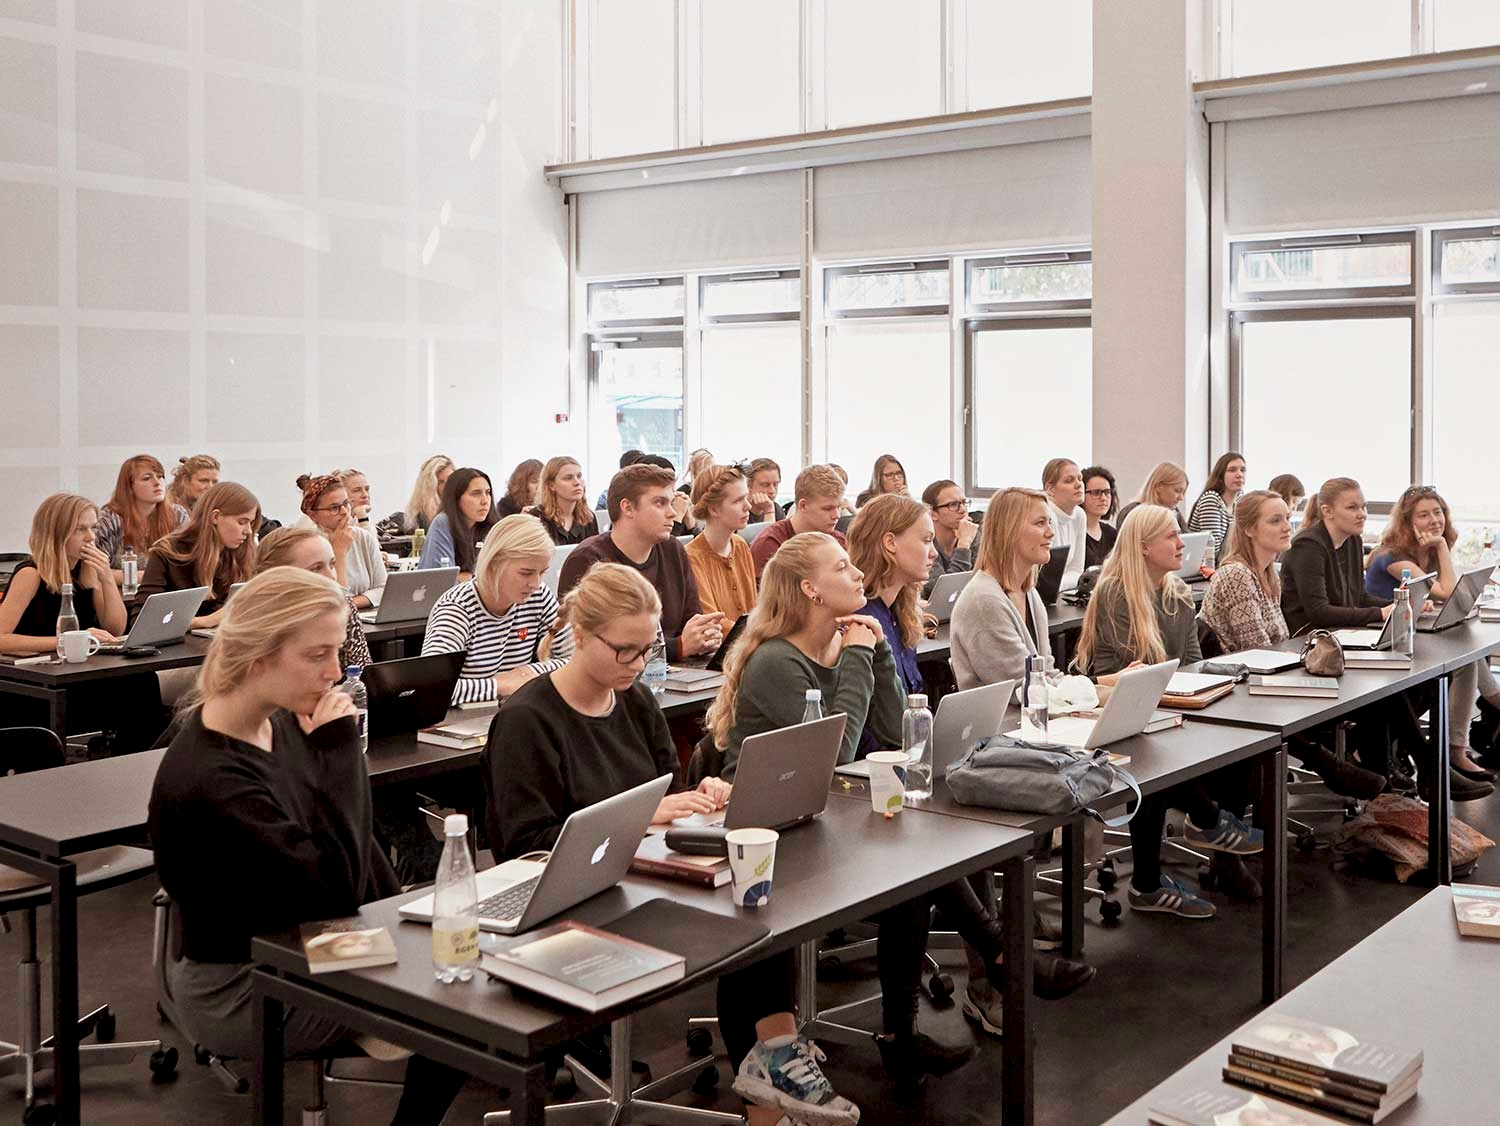
\includegraphics[width=5.1cm,height=6.1cm,keepaspectratio]{images/1.jpg}
    \end{multicols}
\end{frame}

\begin{frame}[hvid]
    \frametitle{Slide med stort billede}
    \vspace{0.5cm}
    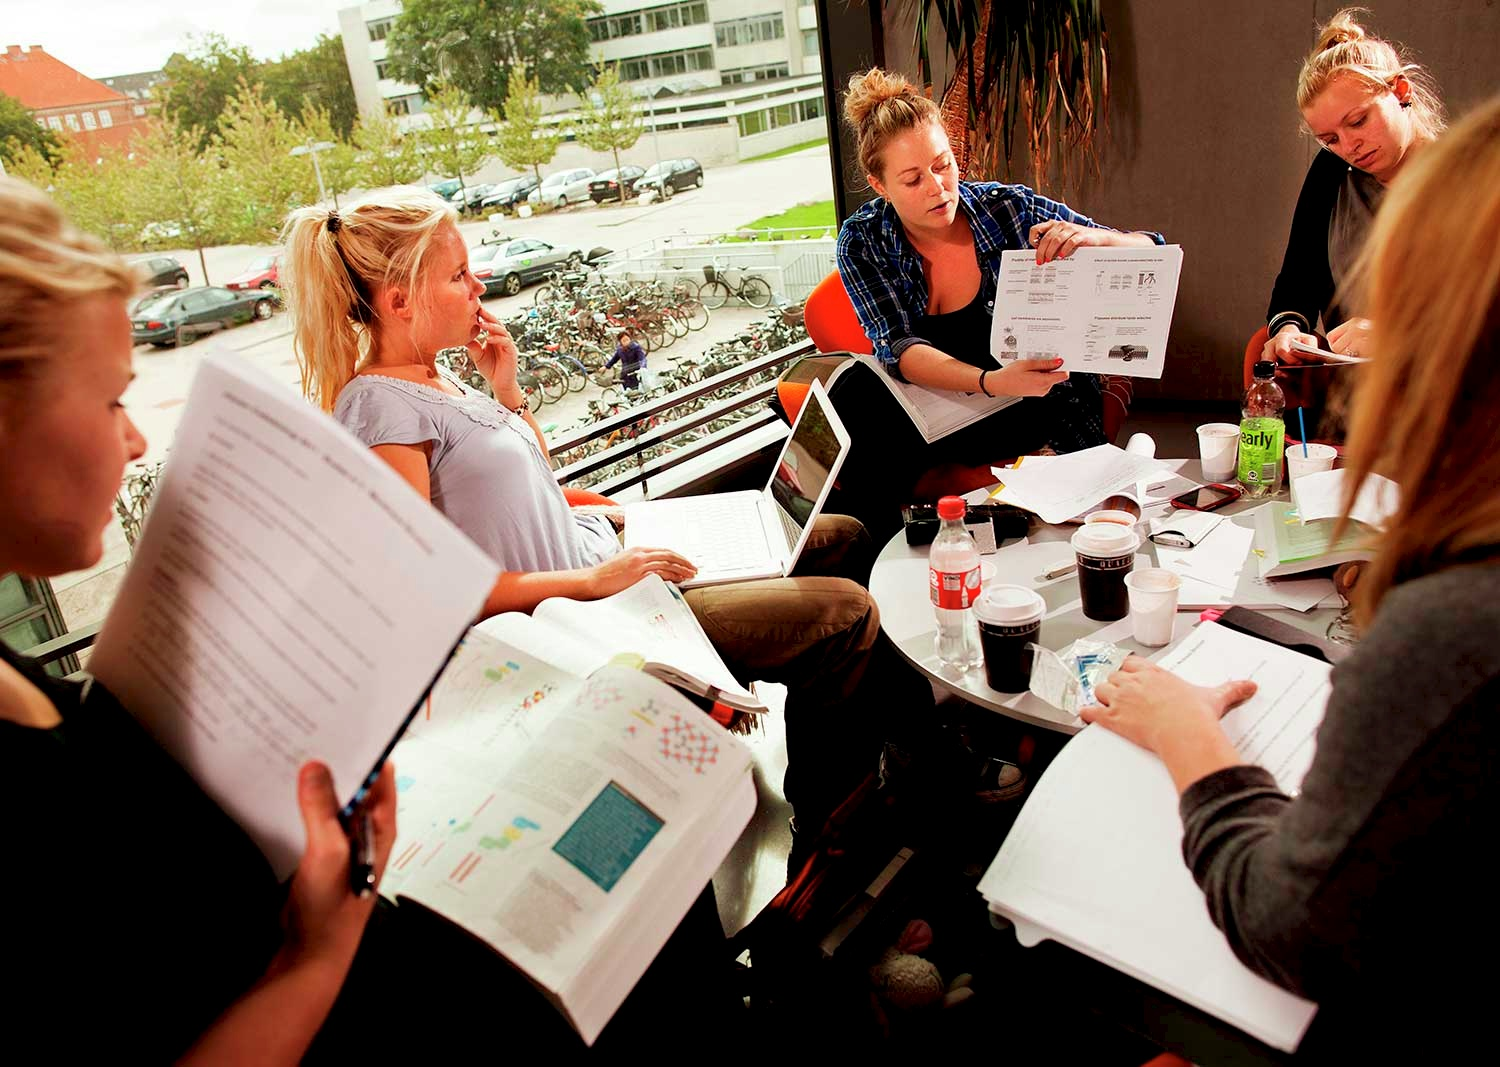
\includegraphics[width=11.3cm,height=6.4cm,keepaspectratio]{images/2.jpg}
\end{frame}

% Her er et eksempel med [billede], hvori man angiver et baggrundsbillede
{
\setbeamertemplate{background}{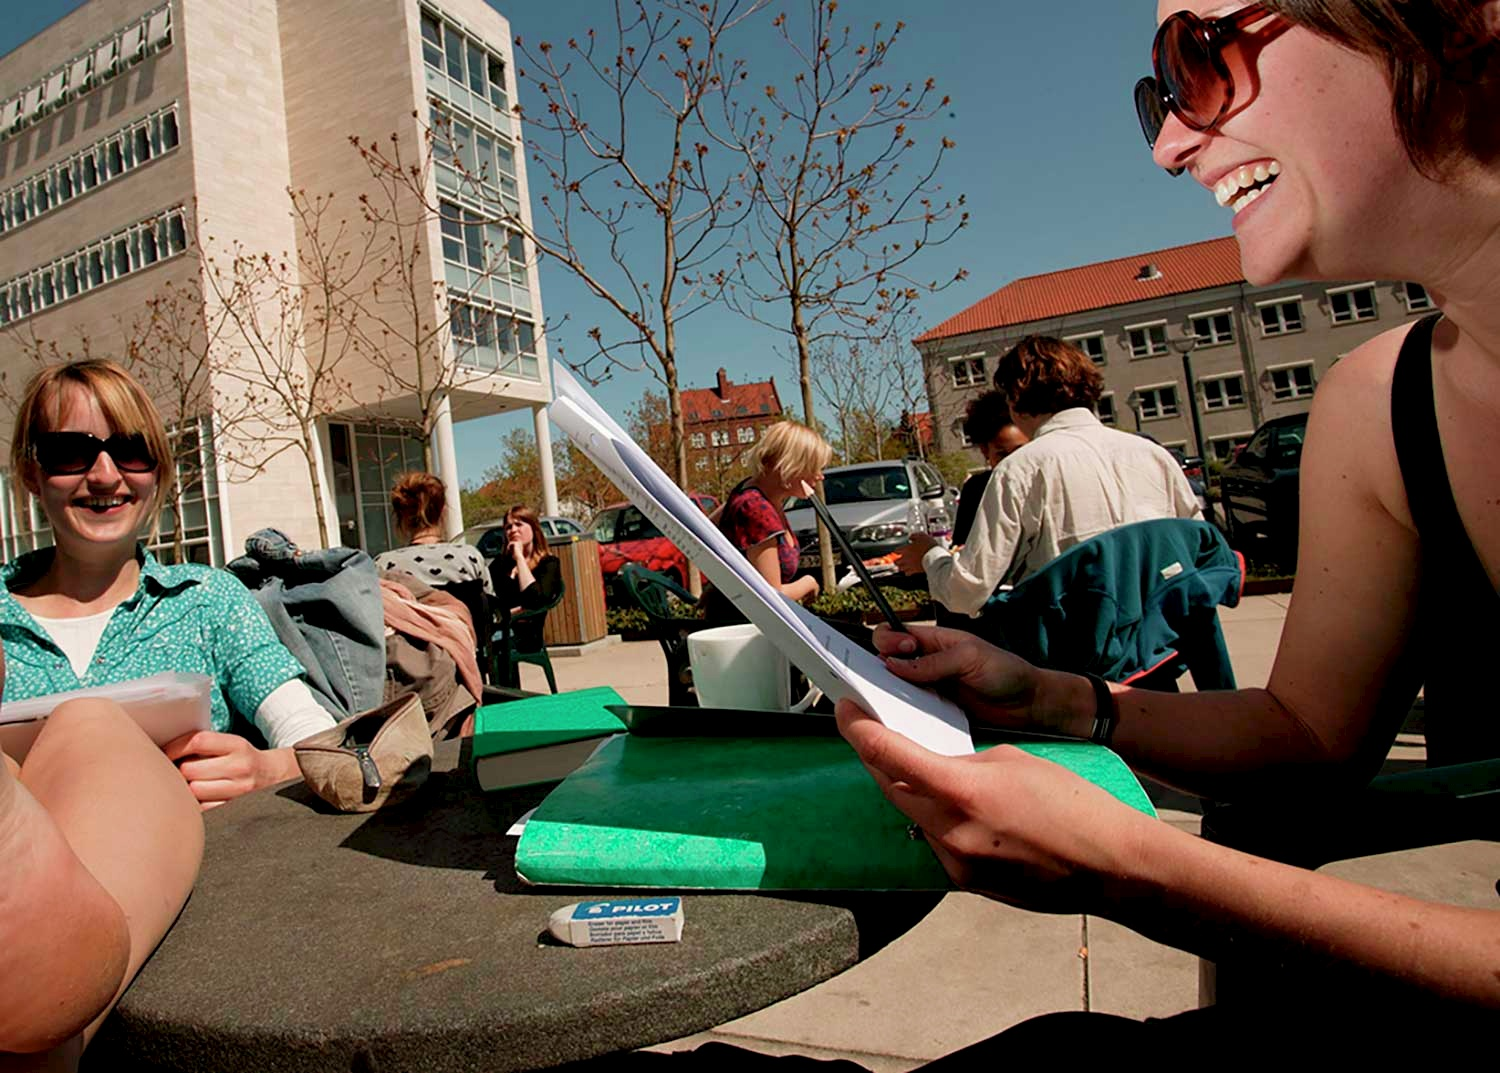
\includegraphics[width=\paperwidth,height=\paperheight]{images/3.jpg}}
\begin{frame}[billede]
    \begin{textblock*}{\textwidth}(0\textwidth,0.77\textheight)
        \begin{beamercolorbox}[wd=6.4cm,sep=0.3cm]{rodbox}
            Et lille mærke med en vilkårlig tekst
        \end{beamercolorbox}
    \end{textblock*}
\end{frame}
}

{
\setbeamertemplate{background}{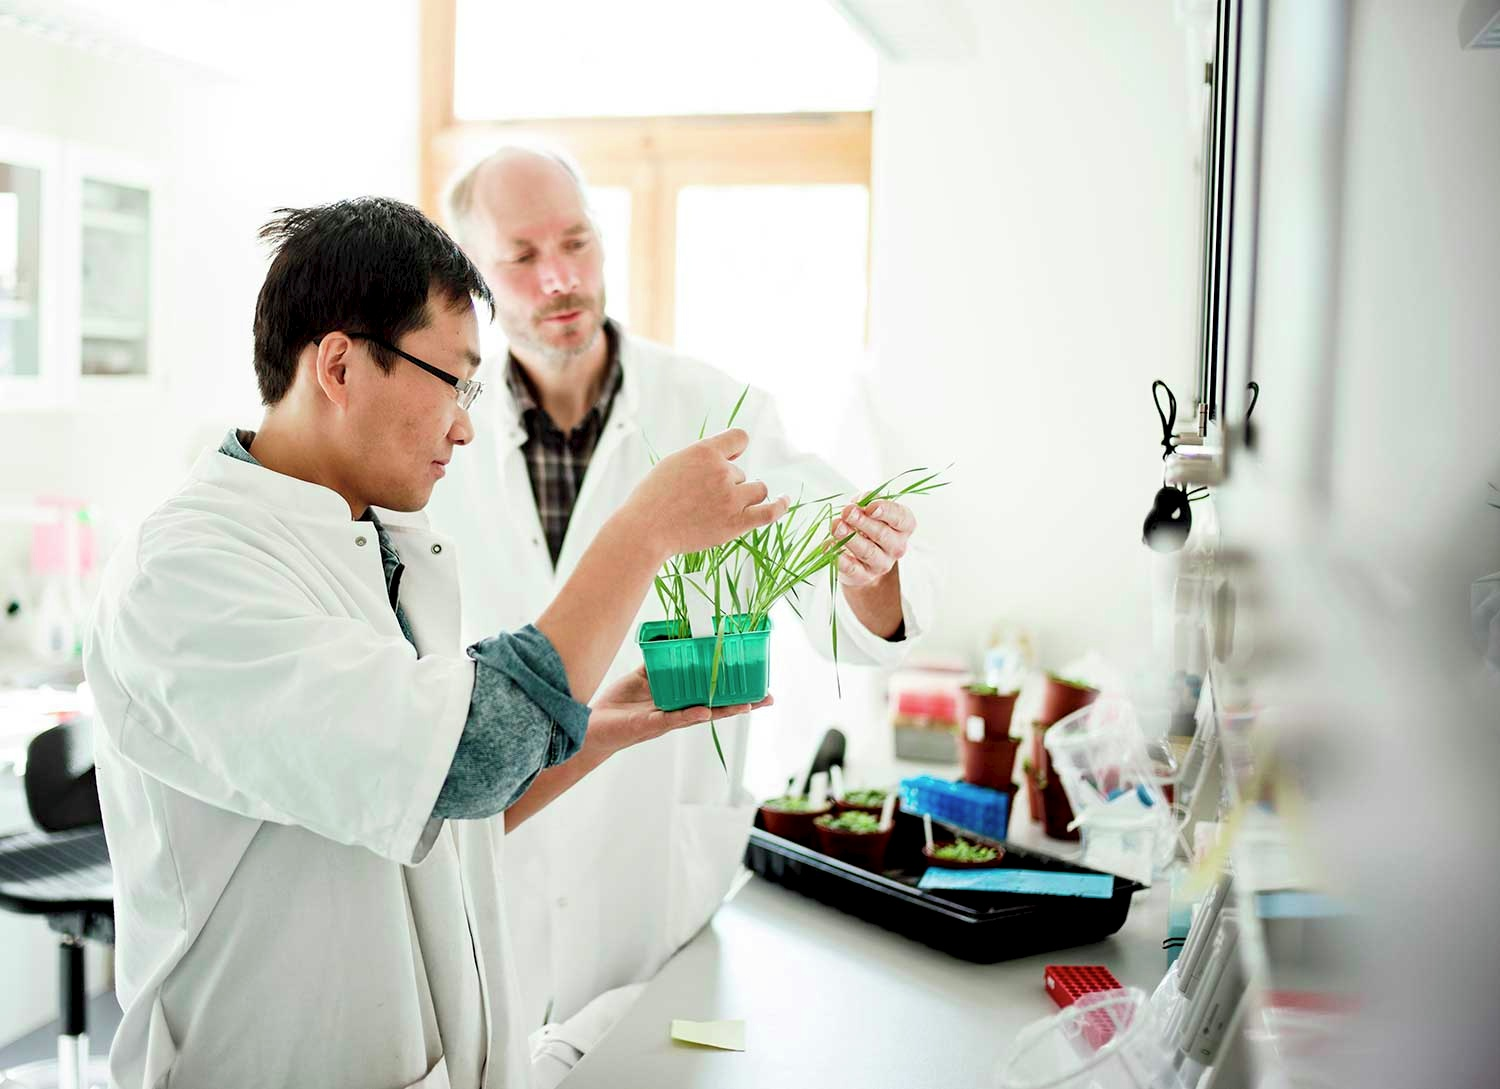
\includegraphics[width=\paperwidth,height=\paperheight]{images/4.jpg}}
\begin{frame}[billede]
    \begin{textblock*}{\textwidth}(0.57\textwidth,0.4\textheight)
        \begin{beamercolorbox}[wd=6.4cm,sep=0.3cm]{rodbox}
            Dette er et stort mærke. Her kan man f.eks. have en liste
            \begin{itemize}
                \item Punkt 1
                \item Punkt 2
                \item Punkt 3
                \item Punkt 4
            \end{itemize}
        \end{beamercolorbox}
    \end{textblock*}
\end{frame}
}

\begin{frame}[rod]
    \fontsize{80}{0}\selectfont ``
    \\
    \vspace{-0.6cm}
    \fontsize{32}{0}\selectfont Prediction is very difficult, especially if it's about the future.
    \\
    \vspace{2.8cm}
    \fontsize{18}{0}\selectfont Niels Bohr
\end{frame}

\begin{frame}[rod]
    \vspace{0.9cm}
    \resizebox{\textwidth}{!}{
        \begin{tabular}{r l}
            \textbf{Research}               & Forskning            \\
            \textbf{Education}              & Uddannelse           \\
            \textbf{Exchange of knowdledge} & Forskningsformidling \\
        \end{tabular}
    }
\end{frame}

\end{document}